\section{Blockchain}
In this section we shall discuss the main ideas of the blockchain system\cite{btc}. The basic unit of currency is defined as a block containing information about a transaction. The transaction is signed using an encrypted signature. The signature requires a private key to generate and a public key for verification. Details of some encryption methods are discussed later. %Direct to that section. 
Once a block signature has been verified, it is considered as a "legal block". To prevent peers from double spending, it is imperative to store all records of previous transactions in the block. This is made possible by storing some information of the previous block in the next block. Further, to ensure the correct chronology of these blocks, a timestamp (epoch) is used in the block, which marks the time of creation of the block. Since each block contains information about the previous block, the timestamp will be linear in the chain. Any discrepancies regarding this is indicative of a fraudulent block. Finally, we come to the main point that is relevant to our work. How does one ensure, in such a decentralized system, that there is no manipulation of information? This is achieved by hashing. Hashing the information in the block produces a 256-bit long hash. It is easy to verify a hash from a block but very difficult to generate a block that produces a given hash\cite{SHA}. Also, changing even a single character can cause a huge change in the hash. Details of hashing are discussed in more detail later %Direct to that section. 
Whether a block should be trusted or not is governed by the concept of "Proof of Work". This involves finding an arbitrary string, called the nonce, by brute-force, to be appended at the end of the block so that its hash starts with a certain minimum number of zeroes. To prevent manipulation of previous transactions, each block starts with the hash of the previous block. Resources in terms of CPU and electricity are used in huge quantities to generate these nonce. Any fraudulent party working individually to manipulate information in the blockchain will be unable to compete in terms of resources to find a proof of work for successive chains. This will in turn ensure that the longest chain is the most trusted one in case of a fork and the other short chains are automatically rejected. Figure \ref{Fig:1} shows the contents of a block. Figure \ref{Fig:2} shows a pictorial representation of a blockchain.\\

\begin{figure}[!htb]
   \begin{minipage}{0.25\textwidth}   
     \centering
     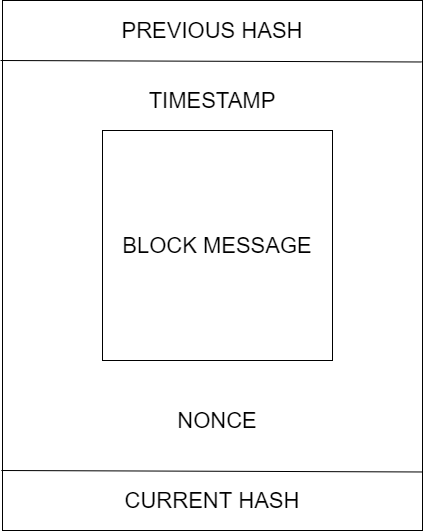
\includegraphics[width=1.1\linewidth]{fig1.png}
     \caption{A typical block}
     \label{Fig:1}
   \end{minipage}\hfill
   \begin{minipage}{0.65\textwidth}
     \centering
     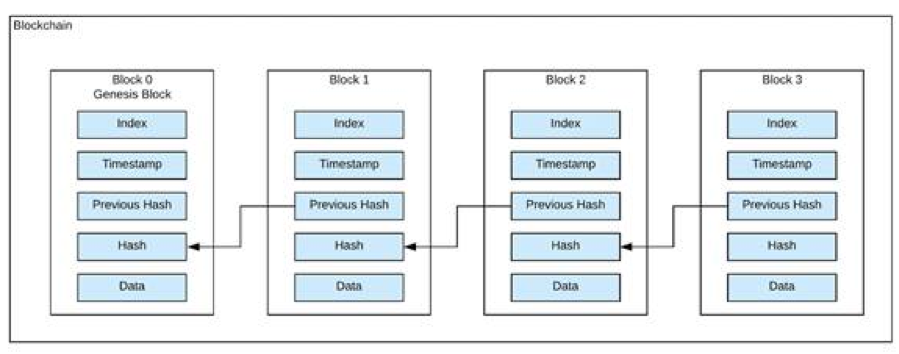
\includegraphics[width=1.1\linewidth]{fig2.png}
     \caption{The structure of a block chain\cite{bcpic}}
     \label{Fig:2}
   \end{minipage}\hfill
\end{figure}

The working of a blockchain system is summarized below.
\begin{enumerate}
\item New transactions are broadcast to all nodes.
\item Each node collects new transactions into a block.
\item Each node works on finding a difficult proof-of-work for its block.
\item When a node finds a proof-of-work, it broadcasts the block to all nodes.
\item Nodes accept the block only if all transactions in it are valid and not already spent.
\item Nodes express their acceptance of the block by working on creating the next block in the
chain, using the hash of the accepted block as the previous hash.
\end{enumerate}

